%%%%%%%%%%%%%%%%%%%%%%%%%%%%%%%%%%%%%%%%%%%%%%%%%%%%%%%%%%%%%%%%%%%%%
% LaTeX Template: Project Titlepage Modified (v 0.1) by rcx
%
% Original Source: http://www.howtotex.com
% Date: February 2014
% 
% This is a title page template which be used for articles & reports.
% 
% This is the modified version of the original Latex template from
% aforementioned website.
% 
%%%%%%%%%%%%%%%%%%%%%%%%%%%%%%%%%%%%%%%%%%%%%%%%%%%%%%%%%%%%%%%%%%%%%%

\documentclass[12pt]{article}
\usepackage[a4paper]{geometry}
\usepackage[myheadings]{fullpage}
\usepackage{fancyhdr}
\usepackage{lastpage}
\usepackage{graphicx, wrapfig, subcaption, setspace, booktabs}
\usepackage[T1]{fontenc}
\usepackage[font=small, labelfont=bf]{caption}
\usepackage[protrusion=true, expansion=true]{microtype}
\usepackage[english]{babel}
\usepackage{sectsty}
\usepackage{url}
\usepackage{lmodern}
\usepackage[utf8]{inputenc}
\usepackage{varioref}
\usepackage {tikz}
\usepackage{float}
\usetikzlibrary {positioning}
\usetikzlibrary{calc}
\usepackage{tabto}
\usepackage{xcolor}
\usepackage{pifont}
\newcommand{\cmark}{\ding{51}}%
\newcommand{\xmark}{\ding{55}}%

\definecolor{DarkGreen}{RGB}{0,140,0}
\definecolor{DarkBlue}{RGB}{0,0,160}
\definecolor{DarkRed}{RGB}{220,0,0}
\definecolor{DarkPurple}{RGB}{160,0,160}

\setlength\parindent{0pt}

\newcommand{\HRule}[1]{\rule{\linewidth}{#1}}
\onehalfspacing
\setcounter{tocdepth}{5}
\setcounter{secnumdepth}{5}

%-------------------------------------------------------------------------------
% HEADER & FOOTER
%-------------------------------------------------------------------------------
\pagestyle{fancy}
\fancyhf{}
\setlength\headheight{15pt}
\fancyhead[L]{Algorithmique Appliquée}
\fancyhead[R]{L. Giovannangeli, F. Jacques, J. Narboni}
\fancyfoot[R]{Page \thepage\ of \pageref{LastPage}}
%-------------------------------------------------------------------------------
% TITLE PAGE
%-------------------------------------------------------------------------------

\begin{document}

\title{ \normalsize \textsc{Algorithmique Appliquée}
		\\ [2.0cm]
		\HRule{0.5pt} \\
		\LARGE \textbf{\uppercase{Projet RoboCup}}
		\HRule{2pt} \\ [0.5cm]
		\normalsize \today \vspace*{5\baselineskip}}

\date{}

\author{
		Loann Giovannangeli, Fabien Jacques, Jonathan Narboni}

\maketitle
\renewcommand{\contentsname}{Sommaire}
\newpage
\tableofcontents
\newpage

%-------------------------------------------------------------------------------
% Section title formatting
\sectionfont{\scshape}
%-------------------------------------------------------------------------------

%-------------------------------------------------------------------------------
% BODY
%-------------------------------------------------------------------------------
\part{Modélisation du Problème}

L'objectif de ce projet est de trouver une modélisation du problème de défense d'un but lors de la ligue SSL de la RoboCup et de l'implémenter. Ce problème consiste à trouver une manière optimale de placer les défenseurs par rapports à l'emplacement de leur but et des attaquants. Nous modéliserons le problème par un graphe. Une solution du problème sera un ensemble dominant de ce graphe.


\section{Entrées}
Les entrées de notre problème sont des informations sur les robots et le terrain :

Soient :
\begin{itemize}
\item $o_i \in O$ ($i \in \{1,..., n\}$) Les $n$ adversaires. On notera $o_i.x$ et $o_i.y$ les coordonnées de $o_i$.
\item $d_i \in D$ ($i \in \{1,..., k\}$) Les $m$ défenseurs.
\item $\theta_{step}$ Pas de discrétisation pour les angles de tirs. On considérera "l'angle $k$" comme étant un angle de mesure $k \cdot \theta_{step}$ radians. On nommera $K_{max}$ le plus grand angle possible, c'est à dire :  $\left \lfloor{\frac{2\cdot p \cdot i }{\theta_{step}}}\right \rfloor $
\item $pos_{step}$, $X_{min}$, $X_{max}$, $Y_{min}$, $Y_{max}$, Pas de discrétisation pour les positions sur le terrain, Abscisses et Ordonnées minimales et maximales.
\end{itemize}

\section{Fonctions nécessaires}
\begin{itemize}
\item $cadre(x, y, k)$ ($x, y, k \in N$) Fonction qui renvoie vrai si le tir d'un attaquant aux coordonnées $(x, y)$ d'angle $k$ est bien cadré et faux sinon.
\item $interception(x, y, k, x', y')$ Fonction qui renvoie vrai si le tir d'un attaquant en (x, y) d'angle k est arrêté par un défenseur en (x', y') et faux sinon.
\end{itemize}
\space
\space

\section{Graphe} \bigbreak
On crée le graphe G suivant :\\
\begin{figure}[H]
	\centering
	\scalebox{1.3}
	{
		
		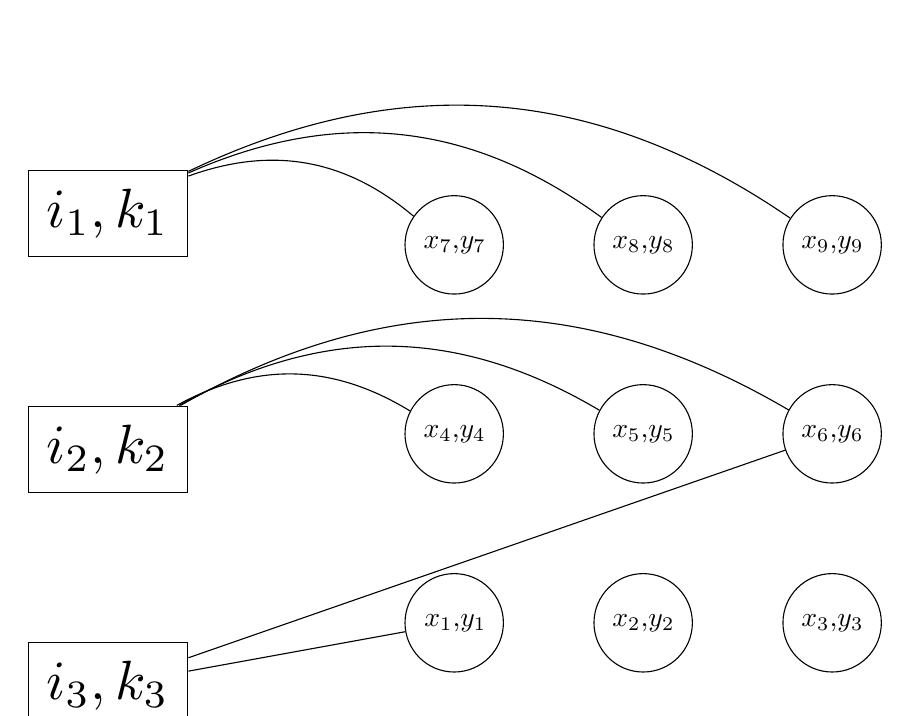
\begin{tikzpicture}[scale=2, transform shape,atq node/.style={shape=rectangle,scale=1,draw=black},def node/.style={scale=0.5, shape=circle,draw=black,inner sep=0,text width=35,align=center}, ]
		\node[atq node] (atq1) at (0,0){$i_3,k_3$};
		\node[atq node] (atq2) at (0,1.5){$i_2,k_2$};
		\node[atq node] (atq3) at (0,3){$i_1,k_1$};
		\newcounter{nDef};
		\setcounter{nDef}{1};
		%def position + basic path
		\foreach \i in {1,...,3}
		{
		    \foreach \j in {1,...,3}
    		{
    		    	\node[def node] (d\arabic{nDef}) at (\j * 1.2 + 1, \i * 1.2 - 0.8){$x_{\arabic{nDef}}$,$y_{\arabic{nDef}}$};
        			\stepcounter{nDef};
    		}
		}
		
		\path (atq1) edge (d1);
		\path (atq1) edge (d6);
		\path (atq2) edge[bend left] (d4);
		\path (atq2) edge[bend left] (d5);
		\path (atq2) edge[bend left] (d6);
		\path (atq3) edge[bend left] (d7);
		\path (atq3) edge[bend left] (d8);
		\path (atq3) edge[bend left] (d9);
		
		\end{tikzpicture}
		
	}
\caption{Exemple de modélisation avec 3 tirs: ici \{($x_6,y_6$), ($x_9,y_9$)\} est une solution.}
\end{figure}
\subsection{Sommets de tir}
On représente chacun des tirs possibles par un sommet (i, k) représentant le tir d'angle k de l'attaquant i :
\newline

$\forall i \in \{1, ..., n\}$, $\forall k \in \{0, ..., K_{max} \}$

Si $cadre(o_i.x, o_i.y, k)$ est vrai : on ajoute un sommet au graphe d'étiquette (i, k) qui représente un tir possible de l'attaquant $o_i$. \bigbreak

\subsection{Sommets de position}
On représente chacune des positions possibles pour un défenseur par un sommet $(x, y)$.
Le fait que se placer à une certaine position permet d'arrêter un tir sera représenté par une arête entre les sommets de tir et de position correspondants.
Les sommets de position reliés à aucun sommet de tir sont retirés du graphe.
Le fait qu'un robot doit se placer à une certaine positions sera représenté par l'appartenance du sommet correspondant à un ensemble dominant.
\newline

$\forall x \in \{1, ..., X_{max}\}$ $\forall y \in \{1, ..., Y_{max}\}$ 

Pour tout sommet d'étiquette (i, k) tel que $interception(o_i.x, o_i.y, k, x, y)$ : On crée un sommet d'étiquette (x, y) qui représente un défenseur placé en (x, y) si ce sommet n'existe pas déjà. Puis, on ajoute une arête entre $(i, k)$ et $(x, y)$ qui représente le fait qu'un défenseur placé en $(x, y)$ arrêterai le tir $(i, k)$.

\section{Solution du problème}
Une solution du problème est un ensemble de taille minimale de sommets de position qui domine(\ref{def:ensemble_dominant}) l'ensemble des sommets de tir . Ceci est effectivement une solution car pour tout sommet de tir on a dans l'ensemble dominant un sommet de position adjacent. En plaçant un défenseur sur chacune des positions dans l'ensemble dominant, tous les tirs possibles des attaquants seront bloqués.

Comme nous sommes limités à 6 robots, nous chercherons des ensemble dominant de tailles entre 1 et 6.

\section{Extensions}
\subsection{Plusieurs buts}
Avec plus de buts, il y a plus de tirs bien cadrés possibles. Cela augmente donc le nombre de sommets de tirs. Il faut modifier la fonction $cadre()$ pour gérer cette extension.

\subsection{Position initiale des défenseurs}

Nos défenseurs ont désormais des coordonnées d'origine (positions initiale) et une solution du problème est une position à atteindre pour chacun des défenseurs. Une solution optimale sera une solution qui permet d'arrêter tous les tirs et qui minimise la distance maximale entre la position initiale d'un défenseur et sa position à atteindre.

\subsection{Distance minimale entre les robots}
Si on veut éviter d'avoir des robots qui rentrent en collision, on peut ajouter une arête entre chaque paire de sommets de position qui ont des positions inférieures à une certaine distance. Une solution du problème doit alors avoir comme condition supplémentaire d'être un ensemble de sommets indépendant (\ref{def:ensemble_de_sommets_indépendant}).\\
Le graphe du problème devient alors :\\ \bigbreak
\begin{figure}[H]
	\centering
	\scalebox{1.3}
	{
		
		\begin{tikzpicture}[scale=2, transform shape,atq node/.style={shape=rectangle,scale=1,draw=black},def node/.style={scale=0.5, shape=circle,draw=black,inner sep=0,text width=35,align=center}, ]
		\node[atq node] (atq1) at (0,0){$i_3,k_3$};
		\node[atq node] (atq2) at (0,1.5){$i_2,k_2$};
		\node[atq node] (atq3) at (0,3){$i_1,k_1$};
		\setcounter{nDef}{1};
		%def position + basic path
		\foreach \i in {1,...,3}
		{
		    \foreach \j in {1,...,3}
    		{
    		    	\node[def node] (d\arabic{nDef}) at (\j * 1.2 + 1, \i * 1.2 - 0.8){$x_{\arabic{nDef}}$,$y_{\arabic{nDef}}$};
        			\stepcounter{nDef};
    		}
		}
		
		\path (atq1) edge (d1);
		\path (atq1) edge (d6);
		\path (atq2) edge[bend left] (d4);
		\path (atq2) edge[bend left] (d5);
		\path (atq2) edge[bend left] (d6);
		\path (atq3) edge[bend left] (d7);
		\path (atq3) edge[bend left] (d8);
		\path (atq3) edge[bend left] (d9);
		
		\path (d1) edge (d4);
		\path (d4) edge (d7);
		\path (d2) edge (d5);
		\path (d5) edge (d8);
		\path (d3) edge (d6);
		\path (d6) edge (d9);
		
		\path (d1) edge (d2);
		\path (d2) edge (d3);
		\path (d4) edge (d5);
		\path (d5) edge (d6);
		\path (d7) edge (d8);
		\path (d8) edge (d9);
		
		\end{tikzpicture}
		
	}
\caption{Exemple de modélisation avec 3 tirs et des collisions : ici \{($x_6,y_6$), ($x_9,y_9$)\} n'est pas une solution mais \{($x_6,y_6$), ($x_7,y_7$)\} est une solution}
\end{figure}

\subsection{Gardien}
Pour modéliser le fait qu'une zone du terrain est réservée à un gardien, on divise les sommets de position en deux : Les sommets de positions terrain $V_{pt}$ et les sommets de position surface de réparation $V_{ps}$ avec $V_p = V_{pt} \cup V_{ps}$  Une solution du problème deviendra donc un ensemble composés de sommets de positions terrain et d'un seul sommet de position surface de réparation qui domine les sommets de tirs.

\section{Limites du modèle}

Ce modèle possède l'avantage de ramener le problème de placement des défenseurs à un problème bien connu, le problème de domination. Cependant, ce modèle est une simplification de la réalité. Voici une liste non-exhaustive des raisons pour lesquels ce modèle est une représentation imparfaite de la réalité :

\begin{itemize}
    \item Chaque attaquant peut tirer en direction des cages. Dans la réalité, seul un attaquant possédant la balle pourrait tirer.
    \item Le vitesse de déplacement de la balle n'est pas pris en compte, dans notre modèle le tir est instantané. Dans la réalité, un défenseur mal placé selon notre modèle pourrait quand même arrêter la balle en se déplaçant sur sa trajectoire avant qu'elle n'arrive dans les cages.
    \item La balle est considérée comme un point sans diamètre.
    \item La trajectoire des attaquants n'est pas prise en compte, seulement leur position actuelle.
\end{itemize}
\part{Résolution du problème}

On a désormais un graphe dont on veut dominer les sommets de tir à l'aide des sommets de position. Pour résoudre ce problème nous avons utilisé les trois approches suivantes :

\section{Force brute}

La premier algorithme que nous avons implémenté est un algorithme de force brute. L'idée est d'essayer exhaustivement tous les sous-ensembles possibles de sommets défenseurs pour en trouver un de taille minimale qui domine les sommets de position. Pour être certain de trouver un sous-ensemble de taille minimale, on commence par essayer tous les sous-ensembles de taille 0, puis 1, puis 2, jusqu'à 6. Si on ne trouve pas d'ensemble dominant durant ce procédé c'est qu'il n'existe pas de solution au problème.\newline\newline

\fbox{\begin{minipage}{\textwidth}
    \centerline{\textbf{Force Brute}}\vspace{\baselineskip}
    
    \textbf{Entrées : }Un graphe $G = (V = V_t \cup V_p, E)$
    
    \textbf{Sortie : }Un ensemble $D \subseteq V_p$ de taille minimale qui domine $V_t$ ou FAUX si un tel ensemble de taille inférieure à 7 n'existe pas. \vspace{\baselineskip}
    
    \textbf{Algorithme :}
    
    \textbf{Pour} $i$ allant de $0$ à $6$ :
    
    \qquad \textbf{Pour} tout $D \subseteq V_p$ avec $|D| = i$ :
    
    \qquad\qquad \textbf{Si} $D$ domine $V_t$ : \textbf{Renvoyer} D \vspace{\baselineskip}
    
    \textbf{Renvoyer} FAUX
\end{minipage}}
\bigbreak
Cet algorithme a une complexité exponentielle pour le nombre de sommets du graphes. En effet, le nombre de sous-ensembles de taille $k$ d'un ensemble à $n$ éléments est exponentiel en $n$.

\subsection{Distance minimale entre les robots}

Pour cette extension, il faut que l'ensemble dominant renvoyé soit également un ensemble indépendant. \newline

\fbox{\begin{minipage}{\textwidth}
    \centerline{\textbf{Force Brute : Distance minimale entre les robots}}\vspace{\baselineskip}
    
    \textbf{Entrées : }Un graphe $G = (V = V_t \cup V_p, E)$
    
    \textbf{Sortie : }Un ensemble $D \subseteq V_p$ de taille minimale qui domine $V_t$ ou FAUX si un tel ensemble de taille inférieure à 7 n'existe pas. \vspace{\baselineskip}
    
    \textbf{Algorithme :}
    
    \textbf{Pour} $i$ allant de $0$ à $6$ :
    
    \qquad \textbf{Pour} tout $D \subseteq V_p$ avec $|D| = i$ :
    
    \qquad\qquad \textbf{Si} $D$ domine $V_t$ et $D$ indépendant : \textbf{Renvoyer} D \vspace{\baselineskip}
    
    \textbf{Renvoyer} FAUX
\end{minipage}}



\subsection{Gardien}

Pour cette extension, il faut qu'exactement un défenseur se trouve sur la surface de réparation et que les autres se trouvent sur le reste du terrain.\newline

\fbox{\begin{minipage}{\textwidth}
    \centerline{\textbf{Force Brute : Gardien}}\vspace{\baselineskip}
    
    \textbf{Entrées : }Un graphe $G = (V = V_t \cup (V_p = V_{pt} \cup V_{ps}), E)$
    
    \textbf{Sortie : }Un ensemble $D \subseteq V_p$ avec un sommet dans $V_{ps}$ de taille minimale qui domine $V_t$ ou FAUX si un tel ensemble de taille inférieure à 7 n'existe pas. \vspace{\baselineskip}
    
    \textbf{Algorithme :}
    
    \textbf{Pour} $i$ allant de $0$ à $6$ :
    
    \qquad \textbf{Pour} tout $D = \{g\} \cup d$ avec $g \in V_{ps}$, $d \subseteq V_{pt}$ et $|D| = i$ :
    
    \qquad\qquad \textbf{Si} $D$ domine $V_t$ : \textbf{Renvoyer} D \vspace{\baselineskip}
    
    \textbf{Renvoyer} FAUX
\end{minipage}}





\subsection{Position initiale des défenseurs}
Dans cette extension le nombre de défenseur nous est donné ainsi que la position initiale de chacun d'entre eux. Il nous faut trouver un ensemble de positions valide (qui permet d'arrêter tous les tirs) qui minimise la distance maximum parcourue par les joueurs en partant de leur position initiale.

\fbox{\begin{minipage}{\textwidth}
		\centerline{\textbf{Force Brute : Positions initiales des défenseurs}}\vspace{\baselineskip}
		
		\textbf{Entrées : }Un graphe $G = (V = V_t \cup V_p , E)$, $V_{init}\subseteq V_p$
		
		\textbf{Sortie : }Un tuple $D \subseteq V_p$  avec un sommet de taille égale à $|V_{init}|$ qui domine $V_t$ tel que $D$ minimise $N_\infty(V_{init},D)$ pour les $D$ dominant $V_t$ tel que $|D|=|V_{init}|$
		
		\textbf{Algorithme :}
		
		 $Liste\_Dominant := \emptyset$
		
		 \textbf{Pour} tout $D_i\subseteq V_t$ tel que $|D|=|V_{init}|$
		
		\qquad \textbf{Si} $D$ domine $V_t$ : Ajouter $D_i$ à $Liste\_Dominant$.
		
		 $D := premierElement(Liste\_Dominant)$.
		
		 \textbf{Si} $Liste\_Dominant = \emptyset$ : \textbf{Renvoyer} FAUX
		
		\textbf{Pour} tout $D_i\in Liste\_Dominant$
		
		\qquad\textbf{Pour} toutes les permutations $\sigma_j\ de\ D_i$
		
		\qquad\qquad\textbf{Si} $N_\infty(V_{init},D_{i,\sigma_j})<N_\infty(V_{init},D)$ : $D:=D_{i,\sigma_j}$.
		
		\textbf{Renvoyer} D
\end{minipage}}
\bigbreak
L'on test ici de manière exhaustive toutes les possibilité d'ensemble dominant $V_t$, ainsi que toutes les permutations possibles pour chaque ensemble. On en déduit l'ensemble dominant ainsi que les positions minimisant la distance maximum parcourue par les défenseurs.

\section{Méthode gloutonne}

Avec cette méthode il est possible d'obtenir une solution avec un nombre de défenseur raisonnablement petit (mais pas minimal) en temps polynomial.\newline

\fbox{\begin{minipage}{\textwidth}
    \centerline{\textbf{Méthode Gloutonne}}\vspace{\baselineskip}
    
    \textbf{Entrées : }Un graphe $G = (V = V_t \cup V_p, E)$
    
    \textbf{Sortie : }Un ensemble $D \subseteq V_p$ qui domine $V_t$ ou FAUX si l'algorithme n'arrive pas à trouver un tel ensemble de taille inférieure à 7. \vspace{\baselineskip}
    
    \textbf{Algorithme :}
    
    Construire une copie $G'$ de $G$
    
    \textbf{Pour} $i$ allant de $0$ à $6$ :
    
    \qquad Choisir un sommet $v \in V_p$ de degré maximal dans $G'$
    
    \qquad Supprimer de $G'$ $v$ et tous les sommets de tir reliés à $v$ 
    
    \qquad Ajouter $v$ à l'ensemble $D$
    
    \qquad \textbf{Si} $D$ domine $V_t$ dans $G$ : \textbf{Renvoyer} $D$\newline
    
    \textbf{Renvoyer} FAUX
\end{minipage}}




\vspace{2\baselineskip}

Cet algorithme a une complexité $O(n\cdot m)$ car trouver un sommet de degré maximal, vérifier qu'un ensemble est dominant, créer une copie d'un graphe et supprimer des sommets dans un graphe peuvent tous se faire en $O(n\cdot m)$

\subsection{Distance minimale entre les robots}
Pour cette extension il faut s'assurer de ne pas prendre de sommet de position relié à un sommet déjà dans la solution. Pour cela, à chaque étape on supprime du graphe les voisins du sommet choisi.\newline

\fbox{\begin{minipage}{\textwidth}
    \centerline{\textbf{Méthode Gloutonne : Distance minimale entre les robots}}\vspace{\baselineskip}
    
    \textbf{Entrées : }Un graphe $G = (V = V_t \cup V_p, E)$
    
    \textbf{Sortie : }Un ensemble $D \subseteq V_p$ qui domine $V_t$ ou FAUX si l'algorithme n'arrive pas à trouver un tel ensemble de taille inférieure à 7. \vspace{\baselineskip}
    
    \textbf{Algorithme :}
    
    Construire une copie $G'$ de $G$
    
    \textbf{Pour} $i$ allant de $0$ à $6$ :
    
    \qquad Choisir un sommet $v \in V_p$ de degré maximal dans $G'$
    
    \qquad Supprimer de $G'$ $v$ et tous les sommets reliés à $v$ 
    
    \qquad Ajouter $v$ à l'ensemble $D$
    
    \qquad \textbf{Si} $D$ domine $V_t$ dans $G$ : \textbf{Renvoyer} $D$\newline
    
    \textbf{Renvoyer} FAUX
\end{minipage}}

\subsection{Gardien}
Pour s'assurer d'avoir exactement $1$ défenseur placé sur la surface de réparation, on commence par choisir un sommet de $V_{ps}$ puis on supprime tous les sommets de position de surface de réparation du graphe.\newline

\fbox{\begin{minipage}{\textwidth}
    \centerline{\textbf{Méthode Gloutonne : Gardien}}\vspace{\baselineskip}
    
    \textbf{Entrées : } Un graphe $G = (V = V_t \cup (V_p = V_{pt} \cup V_{ps}), E)$
    
    \textbf{Sortie : }Un ensemble $D \subseteq V_p$ qui domine $V_t$ ou FAUX si l'algorithme n'arrive pas à trouver un tel ensemble de taille inférieure à 7. \vspace{\baselineskip}
    
    \textbf{Algorithme :}
    
    Construire une copie $G'$ de $G$ \newline
    
    Choisir un sommet $v \in V_{ps}$ de degré maximal dans $G'$
    
    Supprimer de $G'$ v et tous les sommets de tir reliés à $v$
    
    Supprimer de $G'$ les sommets de $V_{ps}$
    
    Ajouter $v$ à l'ensemble $D$
    
    \textbf{Si} $D$ domine $V_p$ dans $G$ : \textbf{Renvoyer} $D$\newline
    
    \textbf{Pour} $i$ allant de $2$ à $6$ :
    
    \qquad Choisir un sommet $v \in V_p$ de degré maximal dans $G'$
    
    \qquad Supprimer de $G'$ $v$ et tous les sommets de tir reliés à $v$  
    
    \qquad Ajouter $v$ à l'ensemble $D$
    
    \qquad \textbf{Si} $D$ domine $V_t$ dans $G$ : \textbf{Renvoyer} $D$\newline
    
    \textbf{Renvoyer} FAUX
\end{minipage}}


\subsection{Position initiale des défenseurs}

\fbox{\begin{minipage}{\textwidth}
		\centerline{\textbf{Méthode gloutonne : Positions initiales des défenseurs}}\vspace{\baselineskip}
		
		\textbf{Entrées : }Un graphe $G = (V = V_t \cup V_p , E)$, $V_{init}\subseteq V_p$
		
		\textbf{Sortie : }Un tuple $D \subseteq V_p$  avec un sommet de taille égale à $|V_{init}|$ qui domine $V_t$ tel que $D$ minimise $N_\infty(V_{init},D)$ pour les $D$ dominant $V_t$ tel que $|D|=|V_{init}|$
		
		\textbf{Algorithme :}
		
  		Construire une copie $G'$ de $G$
  		
		\textbf{Pour} $i$ allant de $0$ à $6$ :
		
		\qquad Choisir un sommet $v \in V_p$ de degré maximal dans $G'$
		
		\qquad Supprimer de $G'$ $v$ et tous les sommets de tir reliés à $v$ 
		
		\qquad Ajouter $v$ à l'ensemble $D_0$
		
		\qquad \textbf{Si} $D_0$ ne domine pas $V_t$ dans $G$ : \textbf{Renvoyer} FAUX \newline
		
		$D=D_0$
		
		\textbf{Pour} toutes les permutations $\sigma_j\ de\ D_0$
		
		\qquad\qquad\textbf{Si} $N_\infty(V_{init},D_{0,\sigma_j})<N_\infty(V_{init},D)$ : $D:=D_{0,\sigma_j}$.
		
		\textbf{Renvoyer} D
\end{minipage}
}
\bigbreak
La méthode gloutonne pour le problème avec des défenseurs ayant une position initiale calcul de façon gloutonne un ensemble dominant $V_t$ de taille égale au nombre de défenseurs initiaux. Cependant, le choix de la permutation pour minimiser la distance maximum parcourue par les défenseur est elle sélectionnée via une méthode force brute.

\section{Réduction vers SAT}

La troisième méthode que nous avons utilisé pour résoudre notre problème est une réduction vers le problème SAT(\ref{def:SAT}). Une fois une instance du problème de domination transformée en instance de SAT, il est possible d'utiliser un solveur SAT pour trouver une solution à ce nouveau problème puis de retransformer cette solution en une solution du problème d'origine.\newline 

On cherche ici à coder notre problème de domination par une formule de logique propositionnelle en forme normale conjonctive(\ref{def:forme_normale_conjonctive}) car les solveurs SAT sont plus efficaces sur les formules en FNC.

\vspace{2\baselineskip}

\fbox{\begin{minipage}{\textwidth}
    \centerline{\textbf{Réduction vers SAT}}\vspace{\baselineskip}
    
    \textbf{Entrées : }Un graphe $G = (V = V_t \cup V_p, E)$ et un entier $k$
    
    \textbf{Sortie : }Une formule de logique propositionnelle en FNC satisfaisable s'il est possible de dominer $V_t$ avec $k$ sommets de $V_p$ ou moins\vspace{\baselineskip}
    
    \textbf{Formule :}
    
    On construit la formule suivante : $\phi = \phi_1 \wedge \phi_2$
    \begin{itemize}
        \item $\phi_1$ représente le fait que chaque sommet de tir est adjacent à au moins un sommet
        \item $\phi_2$ représente le fait qu'il ne peut pas y avoir plus de $k$ sommets dans l'ensemble dominant
    \end{itemize}
    
    
    Cette formule porte sur les variables booléenne :
    \begin{itemize}
        \item $x_i$ \Big($0 \leq i \leq |V_p|$\Big) qui représentent le fait que le sommet $i$ appartient à l'ensemble dominant ou non.
        \item $T_{i, j}$ \Big($1 \leq i \leq k$, $ 1 \leq j \leq |V_p|$\Big) variables auxiliaires utilisées dans $\phi_2$
        \item $B_{i, j}$ \Big($1\leq i \leq k$, $ 1 \leq j \leq \lceil log_2(|V_p|) \rceil$\Big) variables auxiliaires utilisées dans $\phi_2$
    \end{itemize}
    
    $$\phi_1 = \bigwedge\limits_{t\in V_t} \Big(\bigvee\limits_{p\in N(t)} x_p \Big) $$
    
    $$\phi_2 = \bigwedge\limits_{i = 1}^n \left[  \Big(\neg x_i \vee T_{1, i} \vee T_{2, i} \vee ... \vee T_{k, i}\Big) \wedge \bigwedge\limits_{g = 1}^k \bigwedge\limits_{j = 1}^{\lceil log_2(|V_p|) \rceil} \Big( \neg T_{g,i} \vee \phi(i, g, j)\Big)\right]$$
    
    Où $\phi(i, g, j)$ représente $B{g, j}$ si le $j$-ième bit de la représentation en binaire de l'entier $i$ avec $\lceil log_2(|V_p|) \rceil$ chiffres est un $1$ et $\neg B{g, j}$ sinon.
    
\end{minipage}}\newline

Le nombre de littéraux dans la formule $\phi_1$ est borné par $|V_p| ^{|V_t|}$  (dans le pire des cas, chaque sommet de tir est relié à tous les sommets de positions). Le nombre de sommets de tirs étant dans le pire des cas $6*K_{max}$, pour un $K_{max}$ fixé, $\phi_1$ est de taille polynomiale. \newline

La formule $\phi_2$ provient de l'article \cite{FG10}. Elle a une taille en $O\Big(k\cdot |V_p| \cdot log_2(|V_p|)\Big)$ et elle introduit  $O\Big(k \cdot |V_p| \Big)$ nouvelles variables.

Cette réduction est donc FPT pour le nombre de sommets en fixant $K_{max}$ (et donc en fixant $\theta_{step}$).
\part{Implémentation}

\section{Structure du programme}
Nous avons implémenté nos algorithmes en java en utilisant la bibliothèque jgrapht pour la gestion des graphes. Voici la structure générale du programme :\newline

\scalebox{0.7} {
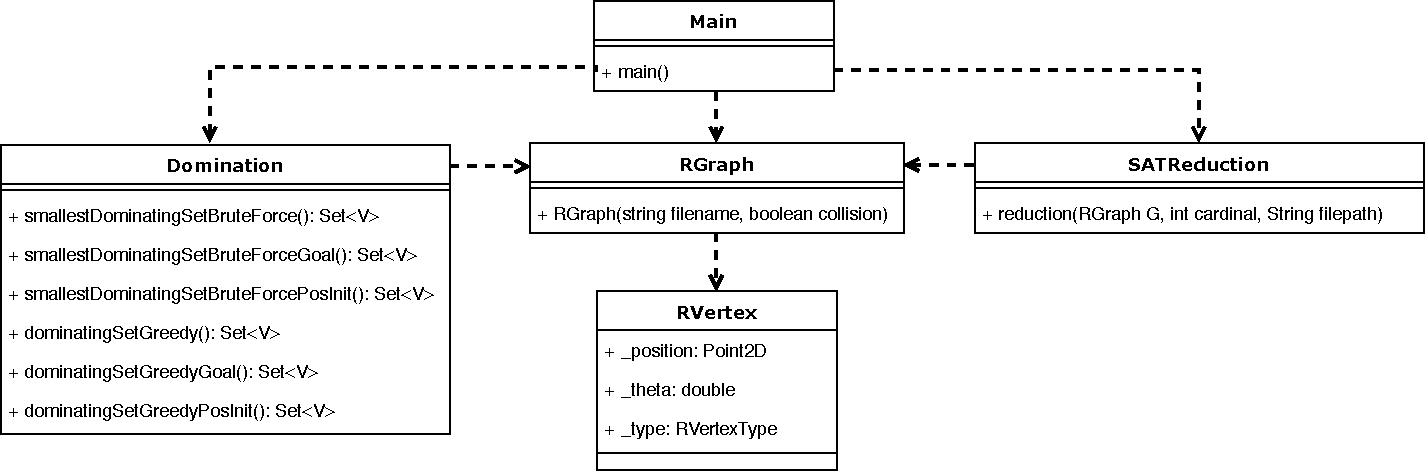
\includegraphics{robotdef.pdf}
} \newline

Le constructeur de la classe RGraph est capable de lire un fichier d'entrée json pour créer un graphe modélisant le problème correspondant. Les sommets de RGraph sont des RVertex. Un RVertex est composé d'une position, d'un angle de tir si le sommet est un sommet de tir et d'un type qui décrit si le sommet est un sommet de tir ou de position (ou un sommet de position surface de réparation dans le cas de l'extension goal). La classe Domination contient les implémentations des algorithmes de résolution et la classe SATReduction la réduction vers SAT. La fonction reduction sauvegarde la formule SAT dans un fichier en format dimacs. Notre programme peut ensuite demander au solveur SAT glucose de tester la satisfaisabilité de cette formule.

\section{Utilisation}

Pour utiliser l'application, compilez tous les fichiers sources dans \textit{robodef/src/main} avec les librairies externes (fichiers .jar) présents dans les dossiers \textit{robotdef/lib\_jgrapht} et \textit{robotdef/lib\_json}.

Lorsque le programme est lancé, vous devez commencer par choisir un fichier au format JSON décrivant le problème dont vous voulez générer une solution (au moins un exemple pour chaque problème est disponible dans le dossier \textit{robotdef/problems}).  Vous devrez ensuite choisir le type de problème (extension) lié au fichier que vous venez de sélectionner.

Le programme utilisera l'algorithme correspondant au type de problème que vous aurez renseigné, sans vérifier la structure du fichier JSON décrivant ce problème. L'utilisation d'un fichier non adapté au problème sélectionné pourrait ne pas donner d'erreur apparente, mais le résultat, s'il en sort un, n'aurait pas de sens.

\subsection{Utilisation de SAT}

L'utilisation de l'algorithme SAT est différent des autres. Pour l'utiliser, il faut tout d'abord aller compiler le code C présent dans \textit{robotdef/glucose-syrup-4.1/simp} avec la commande \textit{make}.

Une fois l'exécutable de glucose généré, vous pouvez lancer notre programme. L'utilisation de SAT ne fonctionne que pour les problèmes normaux (basic problems), il faut donc sélectionner un fichier décrivant un problème de ce type. 

Sélectionnez ensuite SAT


\section{Limitations}

Toutes les extensions n'ont pas été implémentées avec toutes les méthodes. Il n'est pas possible d'utiliser deux extensions en même temps sauf distance minimale qui peut être utilisé en même temps que certaines extensions.

\begin{tabular}{| l | c | c | c | c |}
 \hline		
     & Sans Extension & Plusieurs Buts & Position Initiale & Gardien \\
   \hline 
   Force Brute & 2 & 3 & 4 & 5\\
  \hline  
 Glouton & 2 & 3 & 4  & 5\\
 \hline  
 SAT & 2 & 3 & 4  & 5\\
 \hline  
 Force Brute (Distance Minimale) & 2 & 3 & 4  & 5\\
 \hline  
 Glouton (Distance Minimale) & 2 & 3 & 4  & 5\\
 \hline 
 SAT (Distance Minimale) & 2 & 3 & 4  & 5\\
  \hline  
 \end{tabular}

Nous n'avons pas implémenté le fait de récupérer les positions des défenseurs à partir de la solution renvoyée par glucose. 

\section{Résultats}

La méthode force brute est beaucoup trop lente pour être utilisable lorsque $pos_{step}$ est trop petit (en dessous de $0,4$). \newline

La méthode gloutonne est en revanche très rapide même pour des valeurs de $pos_{step}$ très petites (quelques millisecondes seulement) mais ne donne pas forcément une solution optimale. 
Cependant en pratique la réponse renvoyée par la méthode gloutonne possède généralement le même nombre de défenseurs que la méthode force brute. \newline

La réduction vers SAT permet d'obtenir une solution optimale en un temps beaucoup plus raisonnable. Pour un $pos_{step}$ de $0,2$ la réduction vers SAT prend quelques secondes alors que nous ne savons même pas combien de temps la force brute prendrait pour résoudre ce problème (au moins 30 minutes). Cependant, un temps de réaction de quelques secondes pour une équipe de la robocup serait un désavantage considérable. La méthode gloutonne semble par conséquent plus adaptée.
\begin{appendix}
\section{Définitions}
\subsection{Ensemble dominant}
\label{def:ensemble_dominant}
Un ensemble dominant d'un graphe $G(V, E)$ est un sous ensemble $D \subseteq V$ de sommets tel que tout sommet de $G$ est soit dans $D$ soit adjacent à un sommet de $D$.

\subsection{Nombre de domination}
\label{def:nombre_de_domination}
Le nombre de domination $\gamma(G)$ d'un graphe $G$ est le cardinal d'un plus petit ensemble dominant de $G$.

\subsection{Ensemble de sommets stable}
\label{def:ensemble_de_sommets_stable}
Soit $G(V, E)$ un graphe, un sous-ensemble $S \subseteq V$ de sommets est stable si aucune paire de sommets dans $S$ n'est reliée par une arête de $G$.

\subsection{Problème SAT}
\label{def:SAT}
Le problème SAT ou problème de satisfaisabilité booléenne consiste à déterminer à partir d'une formule de logique propositionnelle(\ref{def:formule_de_logique_propositionnelle}) si il existe ou non une valuation des variables de la formule (une assignation de chacune des variables à VRAI ou FAUX) qui rend la formule vraie.

\subsection{Formule de logique propositionnelle}
\label{def:formule_de_logique_propositionnelle}
Une formule de logique propositionnelle est constituée de variables booléennes (qui peuvent valoir VRAI ou FAUX), d'opérateurs $\vee$ (disjonction ou "ou"), $\wedge$ (conjonction ou "et") et $\neg$ (négation) et de parenthèses. Une telle formule peut être évaluée à VRAI ou FAUX pour une certaine assignation des variables de la formule en suivant certaines règles à appliquer aux opérateurs dans l'ordre défini par les parenthèses. Par exemple $\neg$ FAUX vaut VRAI, FAUX $\vee$ VRAI vaut VRAI...

\subsection{Forme Normale Conjonctive}
\label{def:forme_normale_conjonctive}
Une formule de logique propositionnelle en forme normale conjonctive est constituée de conjonctions de disjonctions de littéraux.
Autrement dit, une formule en FNC a la forme suivante :
$$(l_{1,1} \vee l_{1,2} \vee \ldots \vee l_{1,k_1}) \wedge (l_{2,1} \vee l_{2,2} \vee \ldots \vee l_{1,k_2}) \wedge \ldots \wedge (l_{n,1} \vee l_{n,2} \vee \ldots \vee l_{n,k_n})$$

Où les $l_{i, j}$ sont des littéraux ($x$ ou non $\neg x$ avec $x$ une variable).

\end{appendix}

%Bibliographie
\bibliographystyle{unsrt}
\bibliography{bib}
\nocite{FG10}

%-------------------------------------------------------------------------------
% REFERENCES
%-------------------------------------------------------------------------------
%\newpage
%\section*{References}
%\addcontentsline{toc}{section}{References}

\end{document}
